\documentclass{article} % Tipo de documento

\usepackage[utf8]{inputenc} % Permite el uso de caracteres del Español

\usepackage[T1]{fontenc}

\usepackage{graphicx}

\usepackage{subfig}

% Carátula del Artículo  

\title{Actividad 10}

\author{Roberto Alexis Gomez Pintor}


\begin{document}

\maketitle % Crea el título

\section*{Introduccion}

La teoría del caos es una rama de las matemáticas que trabaja con los sistemas dinámicos no lineales. Un sistema es una serie de componentes que interaccionan para formar un entero mayor. No lineal significa que debido a los efectos multiplicativos de la retroalimentación entre componentes, el total se convierte en algo mayor de la simple suma de sus partes. Finalmente, dinámicos significa que el sistema cambia a lo largo del tiempo basado en su estado actual. Los sistemas caóticos son un subtipo de sistema dinámico no lineal. 

\vspace{0.5 cm}

Para ejemplificar este comportamiento tomemos la curva S de la función logística que muestra el crecimiento de una población. Esta función utiliza una ecuación diferencial que toma al tiempo como un continuo. El mapa logístico en cambio utiliza una ecuación diferencial no lineal reflejando cambios discretos con respecto al tiempo. Este se llama mapa logístico debido a que mapea los valores de población a cualquier lapso de tiempo ligándolo a su próximo lapso de tiempo.

\vspace{0.5 cm}

Esta ecuación define las reglas o dinámicas del sistema, donde X representa la población a un tiempo determinado t, y r representa la tasa de crecimiento. Si la tasa de crecimiento es muy baja, la población morirá. Tasas de crecimiento más altas tenderán a estabilizarse o a tener una serie de aumentos y disminuciones extremos a través del tiempo. A pesar de ser una ecuación simple, para ciertos parámetros de crecimiento se presenta comportamiento caótico. 

\section*{Desarrollo}

Los atractores son valores en los cuales el sistema se debe estabilizar después de un tiempo. Para un sistema en ciertos valores de la tasa de crecimiento no se observa esta estabilización si no que con el tiempo se comienza a observar una tendencia hacia el caos. Un sistema caótico tiene un atractor extraño alrededor del cual el sistema oscilará por siempre, nunca repitiéndose o estableciéndose en un estado fijo o comportamiento estable. Nunca tocará el mismo punto dos veces y su estructura es de tipo fractal. Esto significa que los mismos patrones existen en toda escala sin importar que tanto nos acerquemos al comportamiento. 

Veamos como con distintas condiciones de crecimiento inicial afectan el comportamiento:

\begin{center}

	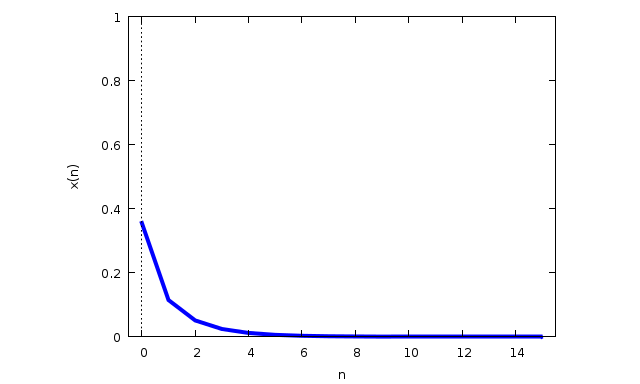
\includegraphics[width=10cm]{1.png}
    
Crecimiento es de 0.5    

\end{center}

\begin{center}

	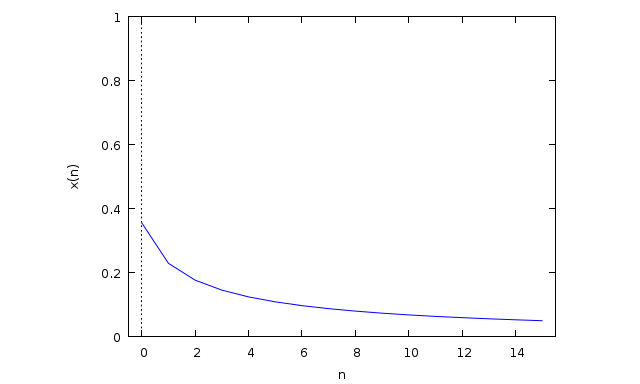
\includegraphics[width=10cm]{2.png}
    
Crecimiento de 1.0

\end{center}

\begin{center}

	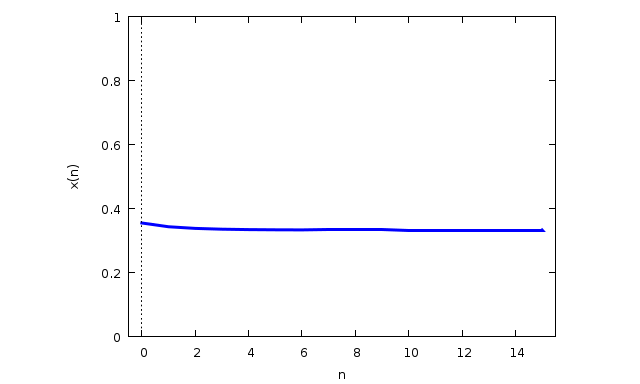
\includegraphics[width=10cm]{3.png}

Crecimiento de 1.5

\end{center}

La imagen muestra varias líneas con los diferentes crecimientos como las anteriores sobrepuestas:

\begin{center}

	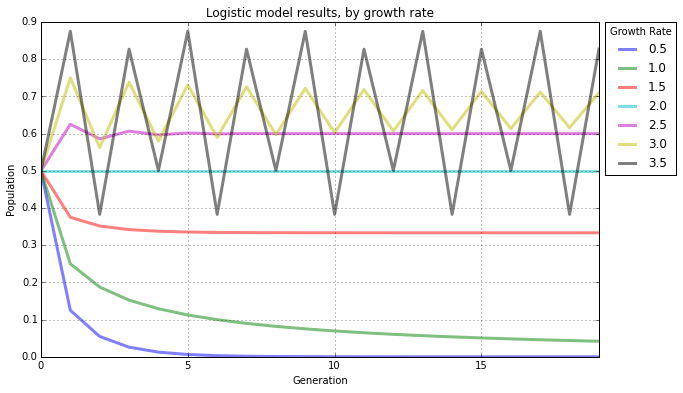
\includegraphics[width=10cm]{logistic-model-line.png}
    
\end{center}


\section*{Bifurcaciones y el camino hacia el caos}

Para crecimientos iniciales menores al 1.0 el sistema siempre tiende a colapsar a cero. Para los crecimientos entre 1.0 y 3.0 el sistema se estabiliza en una población determinada. 

\begin{center}

	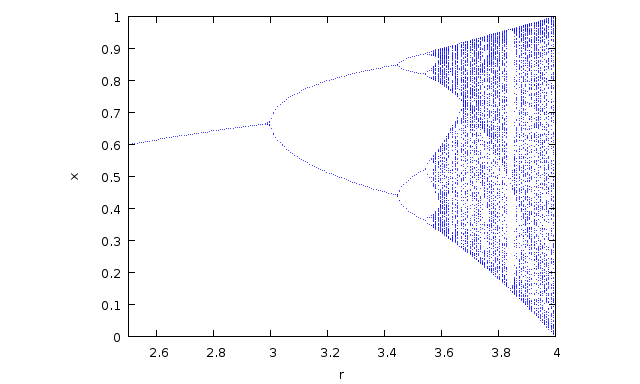
\includegraphics[width=10cm]{4.png}
    
\end{center}

Justo en la tasa de 3.4 y mayores el diagrama inicia a bifurcar en cada vez más caminos. 


\begin{center}

	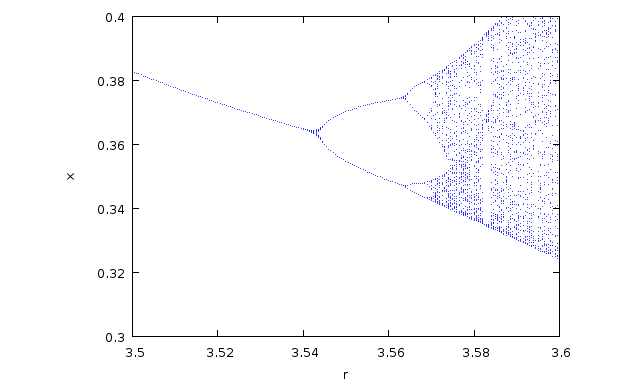
\includegraphics[width=10cm]{5.png}
    
\end{center}


\section*{Inicia el caos}

Más allá de una tasa de crecimiento de 3.6, las bifurcaciones crecerán hasta que el sistema eventualmente caiga en cualquier valor de población. Esto se conoce como el periodo de camino doble del caos. A medida que se ajustan las tasas de crecimiento hacia arriba, el mapa logístico oscilará entre dos, luego cuatro, luego ocho, luego 16 y así sucesivamente, valores de población. Estos como en cualquier péndulo son los periodos de oscilación. Para el momento en que se ha alcanzado la tasa de 3.9, han ocurrido tantas bifurcaciones que el sistema ahora hace brincos, de apariencia aleatoria, entre todos los valores posibles de población. 

\vspace{0.5 cm}

Sin embargo, este comportamiento no es aleatorio, en realidad, este modelo sigue unas reglas deterministas muy simples y aún así produce un comportamiento supuesta-mente errático. Esto es el caos, determinista y no periódico. A medida que nos acercamos al comportamiento podemos ver las bondades del caos. Del ruido emerge una extraña combinación de patrones y niveles en cada uno de los lados en los cuales el sistema se comporta distinto. Entre los valores de 3.82 y 3.84 el sistema se mueve al caos y orden de nuevo, pero después se bifurca hacia el caos en 3.86.


\section*{Atractores extraños}

\begin{center}

	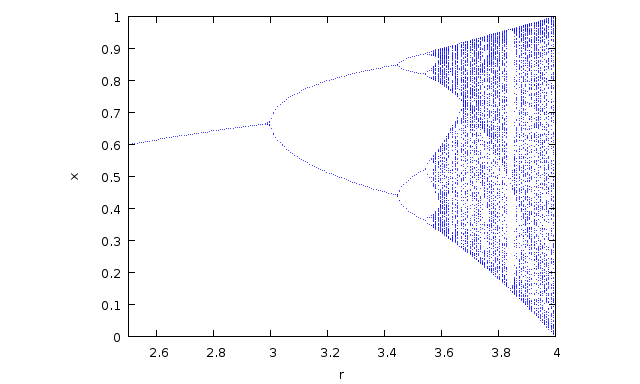
\includegraphics[width=10cm]{6.png}
    
\end{center}

Como se ha mencionado previamente los sistemas caóticos tienen atractores extraños y su estructura se puede caracterizar como un fractal. Los fractales tienen la estructura en cualquier escala en que se observen. A medida que se hace aumento en ellos se encontrarán copias mas pequeñas de la macro-estructura. 


\section*{Caos vs Aleatoriedad}

Los diagramas de fase son útiles para revelar la existencia de atractores extraños en series de tiempo como aquellas generadas por el mapa logístico. Puede resultar difíciles de identificar si ciertas partes del tiempo son caóticas o simplemente aleatorias cuando no se comprenden bien sus dinámicas. 

\begin{center}

	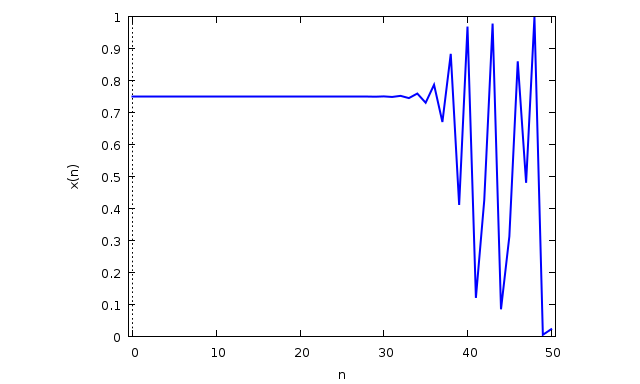
\includegraphics[width=10cm]{7.png}
    
\end{center}


\section*{El efecto mariposa}

Los sistemas caóticos también son clasificados por su alta sensibilidad a las condiciones iniciales. Estos sistemas no tienen una base de atracción que recolecten los puntos cercanos a lo largo del tiempo a un punto fijo o un ciclo límite atractor. En cambio, con un atractor extraño, los puntos cercanos divergen con el tiempo. Esto hace difícil al modelar y predecir en el mundo real, pues se deben medir los parámetros y el estado del sistema con infinita precisión. De lo contrario pequeños errores de medición o redondeo se acumulan con el tiempo y el sistema se desvía totalmente. 

\vspace{0.5 cm}

Fue mediante este tipo de error que Lorenz descubrió el caos. Esto es lo que se conoce comúnmente como el efecto mariposa: "Una mariposa aletea en China y comienza un tornado en Texas". Pequeños eventos se acumulan y afectan el futuro irreversiblemente.

\begin{center}

	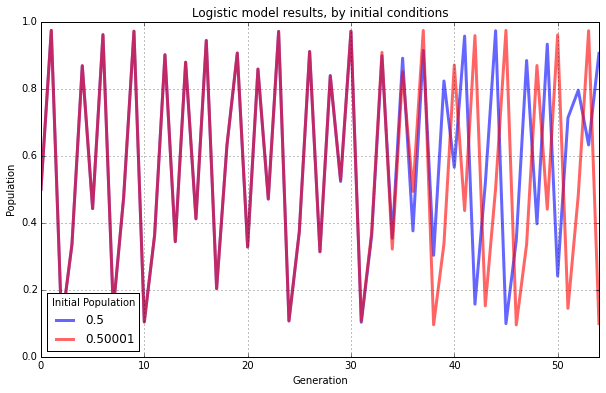
\includegraphics[width=10cm]{mariposa.png}
    
\end{center}

\section*{Las implicaciones del caos}

Ejemplos del mundo real de sistemas caóticos y de tipo fractal incluyen llaves que gotean, el ritmo cardíaco y los generadores de números aleatorios. Muchos expertos han estudiado las implicaciones de la teoría del caos en las ciencias sociales, ciudades y planeación urbana. El caos fundamentalmente indica que existen límites para nuestra capacidad de predicción.          

\vspace{0.5 cm}

Los sistemas deterministas pueden producir comportamientos con bastantes variables y que no se repiten. Cuando se interviene en un sistema se pueden tener resultados impredecibles incluso cuando el cambio es poco, esto se debe a que los efectos se acumulan a lo largo del tiempo. Durante los años 90s, la teoría del caos genero la teoría de la complejidad y prácticamente reemplazo a la primera como un marco analítico para sistemas sociales.  

\vspace{0.5 cm}

La complejidad aborda principios similares pero al final es diferente a la teoría del caos. En lugar de analizar sistemas deterministas simples y cerrados, la teoría de la complejidad examina sistemas grandes y abiertos, conformados por muchas partes en interacción. Bastantes diferentes a los sistemas caóticos, los sistemas complejos mantienen rastros de sus condiciones iniciales y de estados previos por medio de sus "caminos de dependencias".

\end{document}
